\section{Code Quality}
Once the code is in conventional SSA, the correctness problem is solved: destructing it is by definition straightforward, as it relies in renaming all variables in each \phiweb into a unique representative name and then remove all \phifuns. To improve the code however, it
is important to remove as many copies as possible. 

\paragraph{Aggressive coalescing}
This can be treated
with standard non-SSA coalescing technique as conventional SSA allows to get rid of \phifuns: the set of variables of a SSA web can be coalesced leading to a single non-SSA variable; liveness and
interferences can then be defined as for regular code (with parallel copies). An interference graph (as depicted in Figure~\ref{fig:alternative_ssa_destruction:lost-graph}) can be used. A solid edge between two nodes (e.g., between $x_2$ and $x_3$) materialize the presence of an interference between the two corresponding variables, i.e., expressing the fact that they cannot be coalesced and share the same resource. A dashed edge between two nodes materializes an affinity between the two corresponding variables, i.e., the presence of a copy (e.g., between $x_2$ and $x'_2$) that could be removed by their coalescing.

This process is illustrated by Figure~\ref{fig:alternative_ssa_destruction:ex_lost}: the isolation of the \phifun leads to inserting the three copies that respectively define $x'_1$, $x'_3$, and uses $x'_2$; the corresponding \phiweb  $\{x'_1, x'_2, x'_3\}$ is coalesced into a representative variable $x$; according to the interference graph of Figure~\ref{fig:alternative_ssa_destruction:lost-graph}, $x_1$, $x_3$ can then be coalesced with $x$ leading to the code of Figure~\ref{fig:alternative_ssa_destruction:lost3}.

\begin{figure}[H]
\subfloat[Lost-copy problem]{
  \hspace{1em}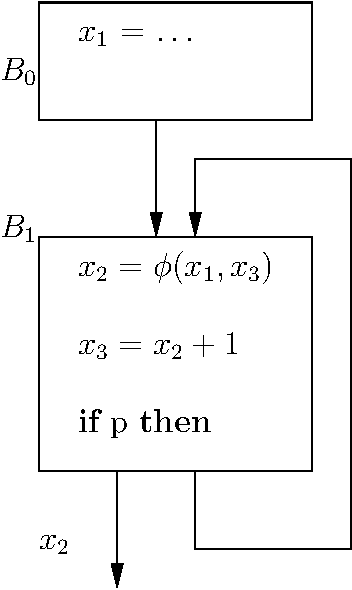
\includegraphics[scale=0.7]{lost.pdf}\hspace{1em}
}
\hfill
\begin{minipage}{0.3\textwidth}
\subfloat[C-SSA]{
  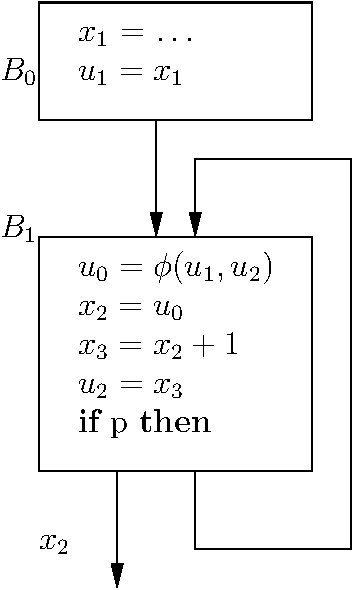
\includegraphics[scale=0.7]{lost2.pdf}
}\\
\subfloat[Interferences\label{fig:alternative_ssa_destruction:lost-graph-cssa}]{
  \hspace{1em}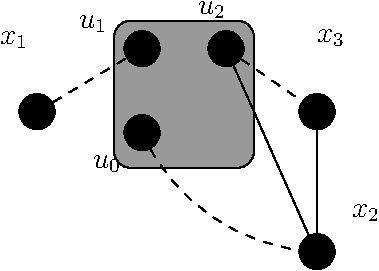
\includegraphics[scale=0.85]{lost-graph-cssa.pdf}\hspace{1em}
}
\end{minipage}
\hfill
\begin{minipage}{0.3\textwidth}
\subfloat[After coalescing\label{fig:alternative_ssa_destruction:lost3}]{
  \hspace{1em}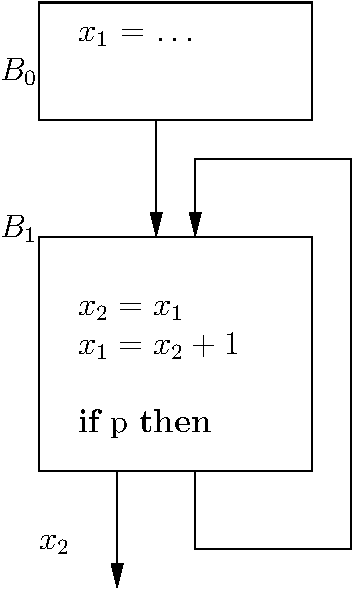
\includegraphics[scale=0.7]{lost3.pdf}\hspace{1em}
}\\\vspace{1em}~\\
\subfloat[Interferences\label{fig:alternative_ssa_destruction:lost-graph}]{
  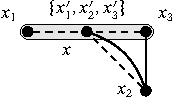
\includegraphics[scale=0.85]{lost-graph.pdf}
}
\end{minipage}
\caption{SSA destruction for the lost-copy problem.\label{fig:alternative_ssa_destruction:ex_lost}}
\end{figure}

\paragraph{Liveness under SSA}
\index{liveness!\phifun}
\label{sec:alternative_ssa_destruction_algorithm:liveness}
If the goal is not to destruct SSA completely but remove as many copies as possible while maintaining the conventional property, liveness of \phifun operands should reproduce the behavior of the corresponding non-SSA code as if the variables of the \phiweb were coalesced all together. The semantic of the \phiop in the so called \emph{multiplexing} mode
fits the requirements. The corresponding interference graph on our example is depicted in Figure~\ref{fig:alternative_ssa_destruction:lost-graph-cssa}.


\begin{definition}[multiplexing mode]
Let a \phifun $B_0:a_0=\phi(B_1:a_1,\dots,B_n:a_n)$ be in \emph{multiplexing} mode, then its liveness follows the following semantic: its \defop is considered to be at the entry of $B_0$, in other words variable $a_0$ is live-in of $B_0$; its \useops are at the exit\index{basic-block exit} of the corresponding predecessor basic-blocks, in other words variable $a_i$ for $i>0$ is live-out of basic-block $B_i$.
\end{definition}



\paragraph{Value-based interference}
\label{par:alternative_ssa_destruction:value}
As said earlier, after the $\phi$-isolation phase and the treatment of operand pining constraints, the code contains many overlapping live-ranges that carry the same value. Because of this, to be efficient coalescing must use an accurate notion of interference.
 % 
\ifhab
It is common to find in the literature the following definition of
  interference ``two variables interfere if their live ranges intersect''
  (e.g.,  in~\cite{George96,liverange.pldi02,SmithRH04}) or its refinement ``two variables interfere if one is live at a definition point of the other'' (e.g., in~\cite{Chaitin82}).  In fact, $a$ and $b$ interfere only if
they cannot be stored in a common register. 
Chaitin et al.  discuss more
  precisely the ``ultimate notion of interference''~\cite{Chaitin81}:
$a$ and $b$
cannot be stored in a common register if there exists an execution point where
$a$ and~$b$ carry {\em two different values} that are both defined, used in the
future, and not redefined between their definition and use.  
%
This definition of interference contains two dynamic (i.e., related to the
execution) notions: the notion of liveness and the notion of value.  
Analyzing statically if a variable is live at a given execution point is a difficult problem. 
This can be approximated (quite accurately in practice) using data-flow reaching definition and upward exposed use~\cite{appel:2002:modern}.  In
strict SSA form -- in which each use is dominated by its unique
definition -- upward exposed use analysis as developed in Chapter~\ref{chapter:ssa_tells_nothing_of_liveness} is sufficient.  The
notion of value is even harder, but may be approximated using data-flow
analysis on specific lattices~\cite{AlpernWZ88, BouchezDEA}.  This has been
extensively studied in particular in the context of partial redundancy
elimination.
The scope of variable coalescing is usually not so large, and
Chaitin proposed a simpler conservative test: \emph{two variables interfere if
  one is live at a definition point of the other and this definition is not a
  copy between the two variables}. This interference notion is the most
commonly used, see for example how the interference graph is computed
in~\cite{appel:2002:modern}.
\else
As already mentioned in Chapter~\ref{chapter:properties_and_flavours} the ultimate notion of interference contains two dynamic (i.e., related to the
execution) notions: the notion of liveness and the notion of value.  
Analyzing statically if a variable is live at a given execution point or if two variables carry identical values is a difficult problem.
The scope of variable coalescing is usually not so large, and graph coloring based register allocation commonly take the following conservative test: \emph{two variables interfere if one is live at a definition point of the other and this definition is not a copy between the two variables}.
\fi

\ifhab
Chaitin et al. noticed that, with this conservative interference definition,
when $a$ and $b$ are coalesced, the set of interferences of the new variable
may be strictly smaller than the union of interferences of $a$ and $b$. Thus,
simply merging the two corresponding nodes in the interference graph is an
over-approximation with respect to the interference definition.  For example,
in a block with two successive copies $b=a$ and $c=a$ where $a$ is defined
before, and $b$ and $c$ (and possibly~$a$) are used after, it is considered that
$b$ and $c$ interfere but that none of them interfere with $a$. However, after
coalescing $a$ and $b$, $c$ should not interfere anymore with the coalesced
variable.
% Noter que dans le cas SSA avec propriété de dominance, il y a toujours une affinité par laquelle on peut attaquer (en effet, si on regroupe toutes les variables reliées par une affinité dans un ensemble, il y en a une qui domine toute les autres. Elle n'interfère pas avec ses fils. Coalescer ses fils à elle c'est juste alonger son live range et garder la définition qui domine comme définition commune. On peut donc itérerer jusqu'à enlever toutes les copies). Ce n'est pas le cas si on est pas sous SSA (multiples définitions).
Hence, the interference graph has to be updated or rebuilt. Chaitin et
al.~\cite{Chaitin81} proposed a counting mechanism, rediscovered
in~\cite{BD3+00}, to update the interference graph, but it was considered to be
too space consuming. Recomputing it from time to time was
preferred~\cite{Chaitin81,Chaitin82}. Since then, most coalescing techniques
based on graph coloring use either live range intersection
graph~\cite{VC+99,liverange.pldi02} or Chaitin's interference graph with
reconstructions~\cite{GA96,BriggsCT94}.
\else
One can notice that, with this conservative interference definition,
when $a$ and $b$ are coalesced, the set of interferences of the new variable
may be strictly smaller than the union of interferences of $a$ and $b$. Thus,
simply merging the two corresponding nodes in the interference graph is an
over-approximation with respect to the interference definition.  For example,
in a block with two successive copies $b=a$ and $c=a$ where $a$ is defined
before, and $b$ and $c$ (and possibly~$a$) are used after, it is considered that
$b$ and $c$ interfere but that none of them interfere with $a$. However, after
coalescing $a$ and $b$, $c$ should not interfere anymore with the coalesced
variable.
Hence the interference graph would have to be updated or rebuilt.
\fi

However, in SSA, each variable has, statically, a \emph{unique} value, given by its unique
definition.  Furthermore, the ``has-the-same-value'' binary relation defined on
variables is, if the SSA form fulfills the dominance property, an equivalence relation.  
The \emph{value} of an equivalence class~\footnote{Dominance property is required here, e.g., consider the following loop body $\textrm{if}(i\neq 0)$ $\{b\gets a;\}$ $c\gets\dots;$ $\dots\gets b;$ $a\gets c;$ the interference between $b$ and $c$ is actual.} 
is the variable whose definition
dominates the definitions of all other variables in the class.
Hence, using the same scheme as in SSA copy folding, finding the value of a
variable can be done by a simple topological traversal of the dominance tree:
when reaching an assignment of a variable $b$, if the instruction is a copy
$b=a$, $V(b)$ is set to $V(a)$, otherwise $V(b)$ is set to $b$. The
interference test in now both simple and accurate (no need to rebuild/update
after a coalescing): if $\textrm{live}(x)$ denotes the set of program points
where $x$ is live, 

\centerline{\emph{$a$ interfere with $b$ if $\textrm{live}(a)$ intersects
  $\textrm{live}(b)$ and $V(a)\neq V(b)$}}

  The first part reduces to
$\textrm{def}(a)\in \textrm{live}(b)$ or $\textrm{def}(b)\in \textrm{live}(a)$
thanks to the dominance property\ifhab~\cite{liverange.pldi02}\fi. In the previous
example, $a$, $b$, and $c$ have the same value $V(c)=V(b)=V(a)=a$, thus they do
not interfere.

Note that our notion of values is limited to the live ranges of SSA
variables, as we consider that each $\phi$-function defines a new variable. We
could propagate information through a $\phi$-function when its arguments are
equivalent (same value). But, we would face the complexity of general value
numbering. By comparison, our equality test in SSA comes for free.

\paragraph{Shared copies}
It turns out that after the $\phi$-isolation phase, and the treatment of operand pining constraints the code also contains what we design as shared copies. A \emph{shared copy} corresponds precisely to the previous example of two successive copies $b=a$ and $c=a$ i.e., the presence of two copies from the same source. 
We have seen that, thanks to our
definition of value, the fact that $b$ is live at the definition of $c$ does
not imply that $b$ and~$c$ interfere.  Suppose however that $a$ (after some
other coalescing) interferes with $b$ and $c$. Then, no coalescing can occur
although coalescing $b$ and $c$ would save one copy, by ``sharing'' the copy of
$a$.  This sharing problem is difficult to model
and optimize (the problem of placing copies is even worse), but we can optimize
it a bit. We coalesce two variables~$b$ and~$c$ if they are both copies of the
same variable~$a$ and if their live ranges intersect. This can be done in a second pass after all standard affinities have been treated. Note that if their live
ranges are disjoint, such a coalescing may be incorrect as it would increase
the live range of the dominating variable, possibly creating some interference
not taken into account.


